\documentclass[14pt,fleqn]{extarticle}
\RequirePackage{prepwell}

\previewoff 

\begin{document} 
\begin{snippet}
    \correct
    
    The figure below shows an ellipse and a circle inside it. 
    $A = (0,1), B = (1,0)$ and $C = (2,0)$ 
    
    \begin{center}
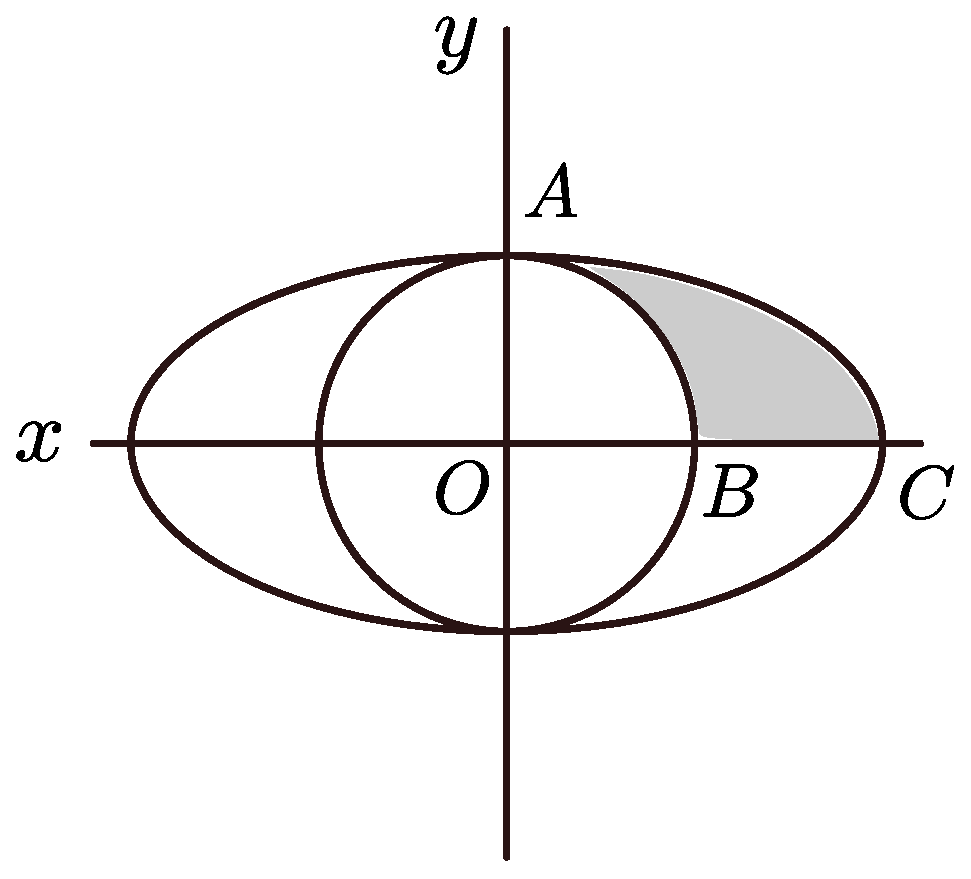
\includegraphics[scale=0.3]{figure.eps}
\end{center}

The shaded portion can therefore be described as 
\small\[ \left\lbrace (x,y) : \cos\theta \leq x \leq 2\cos\theta, y = \sin\theta, \theta \in \left(0,\frac\pi{2}  \right)\right\rbrace\]\normalsize
    
    \reason
    
    You would have noticed that we are working with the parametric forms 
    of equations of a circle and an ellipse 
    
    \begin{center}
  \begin{tabular}{lN}
   \toprule
        &  \text{Parametric Equation} \\
   \midrule 
   Ellipse & x = 2\cos\theta, y = \sin\theta \\
    \midrule 
    Circle & x = \cos\theta, y = \sin\theta \\
    \bottomrule
  \end{tabular}
\end{center}

Any point $(x,y)$ in the shaded region satifies the following conditions 

\begin{center}
  \begin{tabular}{NlN}
   \toprule
        & Condition & \text{Equation} \\
   \midrule 
   x & Beyond the circle & x \geq \cos\theta \\
   & Within ellipse & x \leq 2\cos\theta \\
    \midrule 
    y & Exactly $\sin\theta$ & y = \sin\theta \\
    \midrule 
    \theta & First quadrant only & \theta\in \left(0, \frac{\pi}{2} \right) \\
    \bottomrule
  \end{tabular}
\end{center}

This gives us 
    \small\[ \left\lbrace (x,y) : \cos\theta \leq x \leq 2\cos\theta, y = \sin\theta, \theta \in \left(0,\frac\pi{2}  \right)\right\rbrace\]
    
\end{snippet} 
\end{document} 